%%%%%%%%%%%%%%%%%%%%%%%%%%%%%%%%%%%%%%%%%
% Beamer Presentation
% LaTeX Template
% Version 1.0 (10/11/12)
%
% This template has been downloaded from:
% http://www.LaTeXTemplates.com
%
% License:
% CC BY-NC-SA 3.0 (http://creativecommons.org/licenses/by-nc-sa/3.0/)
%
%%%%%%%%%%%%%%%%%%%%%%%%%%%%%%%%%%%%%%%%%

%----------------------------------------------------------------------------------------
%	PACKAGES AND THEMES
%----------------------------------------------------------------------------------------

\documentclass{beamer}

\mode<presentation> {

% The Beamer class comes with a number of default slide themes
% which change the colors and layouts of slides. Below this is a list
% of all the themes, uncomment each in turn to see what they look like.

%\usetheme{default}
%\usetheme{AnnArbor}
%\usetheme{Antibes}
%\usetheme{Bergen}
%\usetheme{Berkeley}
%\usetheme{Berlin}
%\usetheme{Boadilla}
%\usetheme{CambridgeUS}
%\usetheme{Copenhagen} %nice
\usetheme{Darmstadt} %small subsection name on top
%\usetheme{Dresden}
%\usetheme{Frankfurt} %need to specify frametitle
%\usetheme{Goettingen}
%\usetheme{Hannover}
%\usetheme{Ilmenau}
%\usetheme{JuanLesPins}
%\usetheme{Luebeck}
%\usetheme{Madrid} %standard
%\usetheme{Malmoe}
%\usetheme{Marburg}
%\usetheme{Montpellier}
%\usetheme{PaloAlto}
%\usetheme{Pittsburgh}
%\usetheme{Rochester}
%\usetheme{Singapore}
%\usetheme{Szeged}
%\usetheme{Warsaw}

% As well as themes, the Beamer class has a number of color themes
% for any slide theme. Uncomment each of these in turn to see how it
% changes the colors of your current slide theme.

%\usecolortheme{albatross}
%\usecolortheme{beaver}
%\usecolortheme{beetle}
%\usecolortheme{crane}
%\usecolortheme{dolphin}
%\usecolortheme{dove}
%\usecolortheme{fly}
%\usecolortheme{lily}
%\usecolortheme{orchid}
%\usecolortheme{rose}
%\usecolortheme{seagull}
%\usecolortheme{seahorse}
%\usecolortheme{whale}
%\usecolortheme{wolverine}

%\setbeamertemplate{footline} % To remove the footer line in all slides uncomment this line
%\setbeamertemplate{footline}[page number] % To replace the footer line in all slides with a simple slide count uncomment this line

%\setbeamertemplate{navigation symbols}{} % To remove the navigation symbols from the bottom of all slides uncomment this line
}

\usepackage{graphicx} % Allows including images
\usepackage{booktabs} % Allows the use of \toprule, \midrule and \bottomrule in tables
\usepackage{sansmathaccent}
\pdfmapfile{+sansmathaccent.map}
\usepackage{comment} %comment
%----------------------------------------------------------------------------------------
%	TITLE PAGE
%----------------------------------------------------------------------------------------

\title[]{Apply machine learning to Performance trend analysis} % The short title appears at the bottom of every slide, the full title is only on the title page

\author{Araya Eamrurksiri} % Your name
\institute[] % Your institution as it will appear on the bottom of every slide, may be shorthand to save space
{
 \\ % Your institution for the title page
\medskip
\textit{} % Your email address
}
\date{May 19, 2017} % Date, can be changed to a custom date

\begin{document}

\begin{frame}
\titlepage % Print the title page as the first slide
\end{frame}

\begin{frame}
%\frametitle{Overview} % Table of contents slide, comment this block out to remove it
\tableofcontents % Throughout your presentation, if you choose to use \section{} and \subsection{} commands, these will automatically be printed on this slide as an overview of your presentation
\end{frame}

%----------------------------------------------------------------------------------------
%	PRESENTATION SLIDES
%----------------------------------------------------------------------------------------

\section{Introduction} 
\subsection{Motivation}
\begin{frame}
%\frametitle{Motivation}

\begin{itemize}
	\item Many test cases are executed for testing software packages 
	\item Evaluate how each software package performs for an updated software package
	\item Tool or algorithm that can reduce workload of manual inspection
\end{itemize}	

\end{frame}
%------------------------------------------------
\subsection{Objectives}
\begin{frame}
%\frametitle{Objectives}
\begin{itemize}
	\item Detect the state of the CPU utilization (degrading, improving or steady state)
	\item Detect whether there is any change in the test environment that effects the CPU utilization
\end{itemize}
\end{frame}

%------------------------------------------------
\section{Data}
\subsection{Data sources}
\begin{frame}[fragile]
%\frametitle{Data sources}
\begin{comment}
Software release 
\begin{itemize}
	\item two major releases per year
	\item labeled with L followed a number related to the year of release and a letter A or B
\end{itemize}

Software package
\begin{itemize}
	\item act as a snapshot or marker
	\item labeled with R followed numbers and letters
\end{itemize}
\end{comment}

\begin{itemize}
	\item Software release
	\item Software package - treated as a time point in the time series

	\begin{figure}
		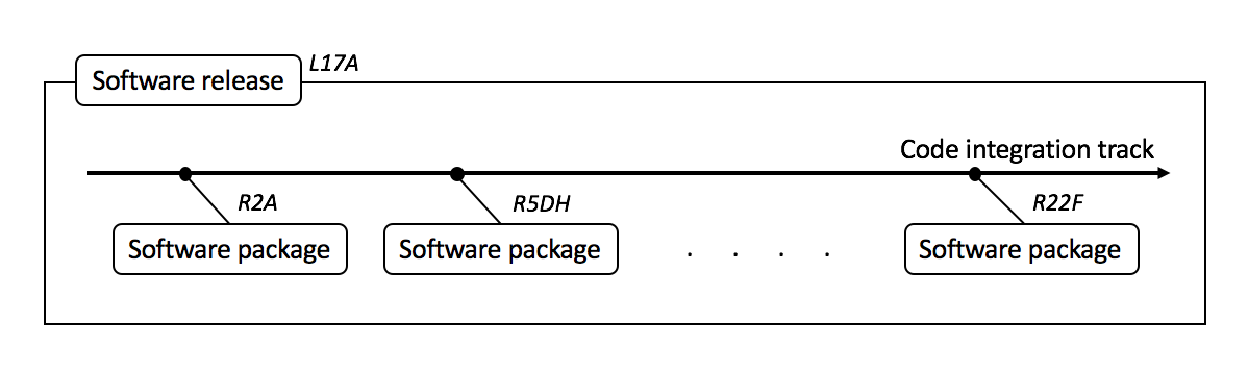
\includegraphics[width=0.8\linewidth]{Release}
		\caption{Several software packages that are launched in the timeline}
	\end{figure}

	\item Test cases \footnotesize{in QA capacity area on signaling capacity} \normalsize{- treated as an observation in the dataset}
\end{itemize}

\end{frame}


%------------------------------------------------
\subsection{Data preprocessing}
\begin{frame}
%\frametitle{Data preprocessing}
Data is collected on January 20, 2017

Three datasets: Software release L16A, L16B, and L17B
\begin{itemize}
	\item Sorted by software package version
	\item Filtered out test cases which are not executed properly
	\item Selected test case which has \textit{lowest} value of the CPU utilization to represent a performance of a specific software package
\end{itemize}

In total, each dataset contains 64, 241, and 144 test cases, respectively

\end{frame}

%------------------------------------------------
\begin{frame}
%\frametitle{Data preprocessing}
EventsPerSec: Event intensity 
\begin{itemize}
	\item Contains several \textit{local events}
	\item Stores multiple values separated by a tab character
	\item Some local events are used as predictor variables
	\item Implement a function to split each element to columns
\end{itemize}

\end{frame}

%------------------------------------------------
\begin{frame}
Response variable 
\begin{itemize}
	\item TotCpu\%: CPU utilization
\end{itemize}	
\vspace{1em}
Predictor vairalbes
\begin{itemize}
	\item EventsPerSec
	\begin{itemize}
		\item RrcConnectionSetupComplete
		\item Paging
		\item X2HandoverRequest
	\end{itemize}	
	\item Test environments
	\begin{itemize}
		\item DuProdName: Product hardware name
		\item Fdd/Tdd: Different standard of LTE 4G Technology
		\item NumCells: Number of cells in the base station
	\end{itemize}
\end{itemize}


\end{frame}

%------------------------------------------------
\section{Method} 
\subsection{Markov switching model}
\begin{frame}
Markov switching model \cite{p1}

Assuming that $S_{t}$ denote an unobservable state variable

$$y_{t} = X_{t}\beta_{S_{t}} + \phi_{1,S_{t}} y_{t-1} + \varepsilon_{t}, \quad \varepsilon_{t} \sim N(0,\sigma^{2}_{S_{t}})$$

$y_{t}$ is the observed value of time series at time $t$ 

$X_{t}$ are the predictor variables of time series at time $t$ 

$\beta_{S_{t}}$ are the coefficients in state $S_{t}$, where $S_{t}=1,2,...,k$

$\phi_{1,S_{t}}$ is an autoregression coefficient of the observed value at time $t-1$ in state $S_{t}$

The observation are drawn from the first order autoregressive model, AR(1).


\begin{figure}
	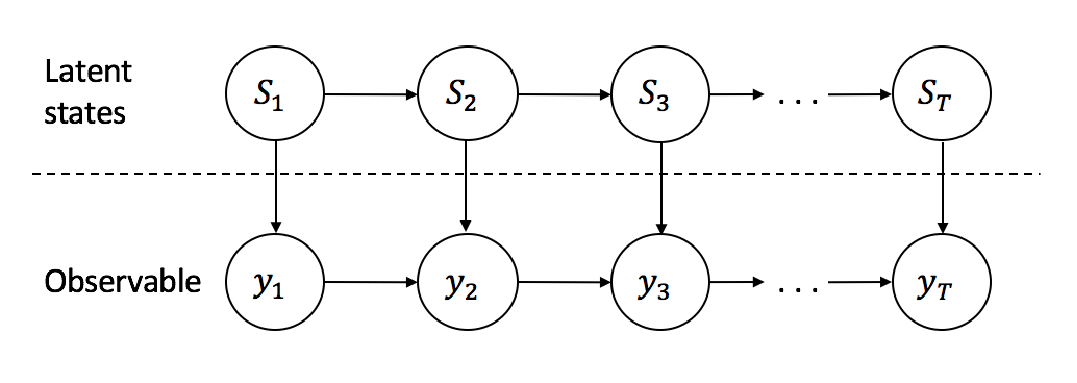
\includegraphics[width=0.5\linewidth]{msm-ar1}
	\caption{Model structure}
\end{figure}

\end{frame}

%------------------------------------------------
\begin{frame}
df
\end{frame}


%------------------------------------------------
\subsection{Model selection}
\begin{frame}
When applying the Markov switching model, we need to decide on
\begin{itemize}
	\item Number of states, $k$
	\item Number of switching coefficients in the model
\end{itemize}
\vspace{1em}

Based on the applied literature, the information criteria called the Bayesian Information Criterion is used to select these numbers

$$\mathrm{BIC}=-2\ln(L(\hat{\theta}))+m\cdot\ln(T)$$


\end{frame}

%------------------------------------------------
\subsection{E-divisive method}
\begin{frame}
E-divisive method \cite{p3}
\begin{itemize}
	\item Non-parametric approach: more flexible as no assumption about the distribution is made
	\item Detects multiple change point locations based on a divisive hierarchical estimation algorithm
	\item Algorithm: 
	
	recursively partition a time series, and perform a permutation test to find the statistical significance of an estimated change point. 
\end{itemize}


\end{frame}

%------------------------------------------------
\subsection{Simulation study for model evaluation}
\begin{frame}
\begin{itemize}
	\item State of the CPU utilization is unknown
	\pause
	
	\item Simulated two datasets - Dataset 1 and Dataset 2 - with different switching between states
\end{itemize}

$$y_{t}=\begin{cases}
	\begin{array}{c}
		10+0.6X_{1,t}-0.9X{}_{2,t}+0.5y_{t-1}+\varepsilon_{t}^{(1)}\\
		2+0.8X_{1,t}+0.2y_{t-1}+\varepsilon_{t}^{(2)}\\
		-12+0.7X_{1,t}+0.2X{}_{2.t}-0.2y_{t-1}+\varepsilon_{t}^{(3)}
	\end{array} & \begin{array}{c}
		\mathrm{Normal}\\
		\mathrm{Bad}\\
		\mathrm{Good}
\end{array}\end{cases}$$

$y_{t}$ is assumed to be a value of a CPU usage of the time series at time $t$

$x_{1,t}\sim U[50,200]$ of the time series at time $t$

$x_{2,t}\sim U[0,50]$ of the time series at time $t$

$\varepsilon_{t}^{(1)}\sim N(0,1),\quad \varepsilon_{t}^{(2)}\sim N(2,0.5),\quad \mathrm{and} \quad \varepsilon_{t}^{(3)}\sim N(1,1)$

\end{frame}

%------------------------------------------------
\section{Results}
\subsection{Analysis I: Number of states}
\begin{frame}
Decide: Number of states

Hypothesis: Markov switching model with \textit{two} or \textit{three} states
\rule{\textwidth}{0.4pt}

\begin{itemize}
	\item BIC is one criteria to select the appropriate model but model output and plot should also be taken into account
	\item \textbf{Three-state} model are chosen for further analysis
	\item Remark: 
	
	Higher number of states $k\geq4$ are more likely to give worse results and were not considered
\end{itemize}

\end{frame}

%------------------------------------------------
\subsection{Analysis II: Number of switching coefficients}
\begin{frame}
\small{Decide: Number of switching coefficients in the model

Hypothesis: test environments is possible to have non-switching effects}
\rule{\textwidth}{0.4pt}

Software release L16A

Model with Fdd/Tdd and Numcells are non-switching coefficients


\begin{figure}
	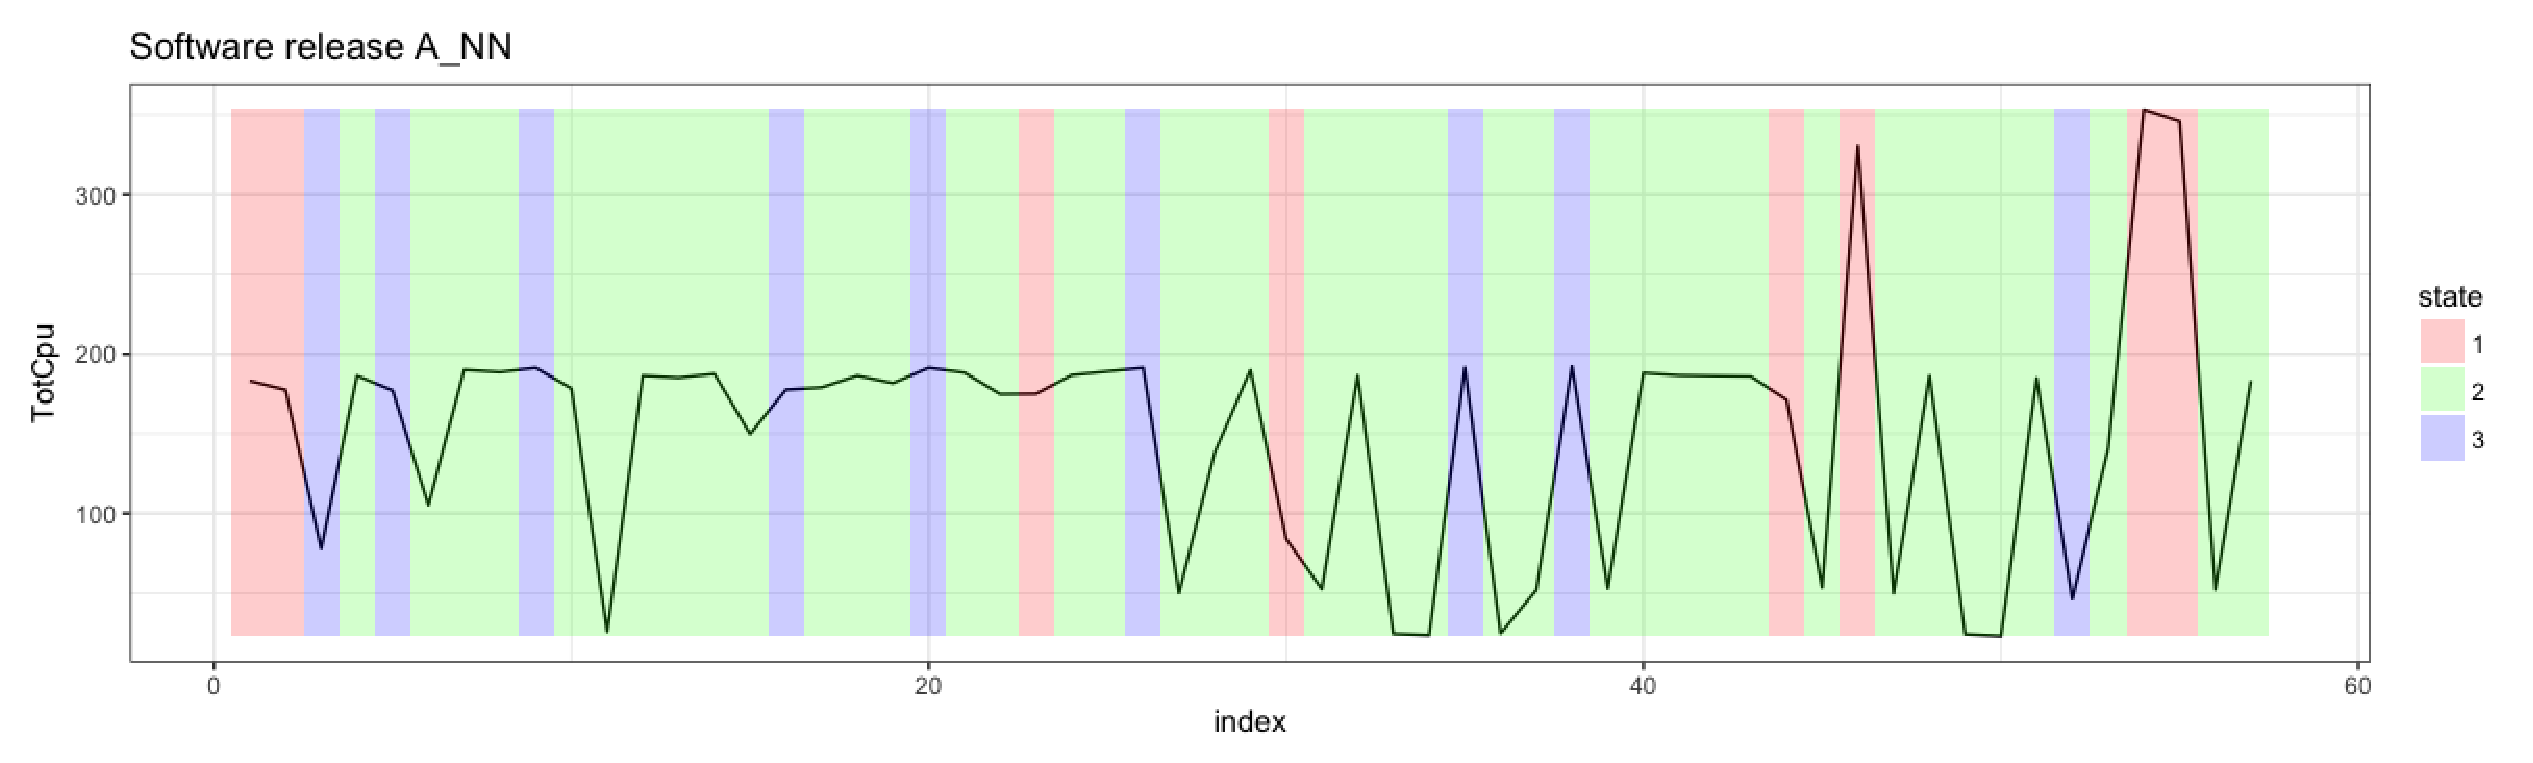
\includegraphics[width=1\linewidth]{L16A_NN1}
	\caption{The CPU utilization showing the periods where the observation is in the specific state.}
\end{figure}


\end{frame}

%------------------------------------------------
\begin{frame}
\small{Decide: Number of switching coefficients in the model
	
Hypothesis: test environments is possible to have non-switching effects}
\rule{\textwidth}{0.4pt}

Software release L16B

\begin{figure}
	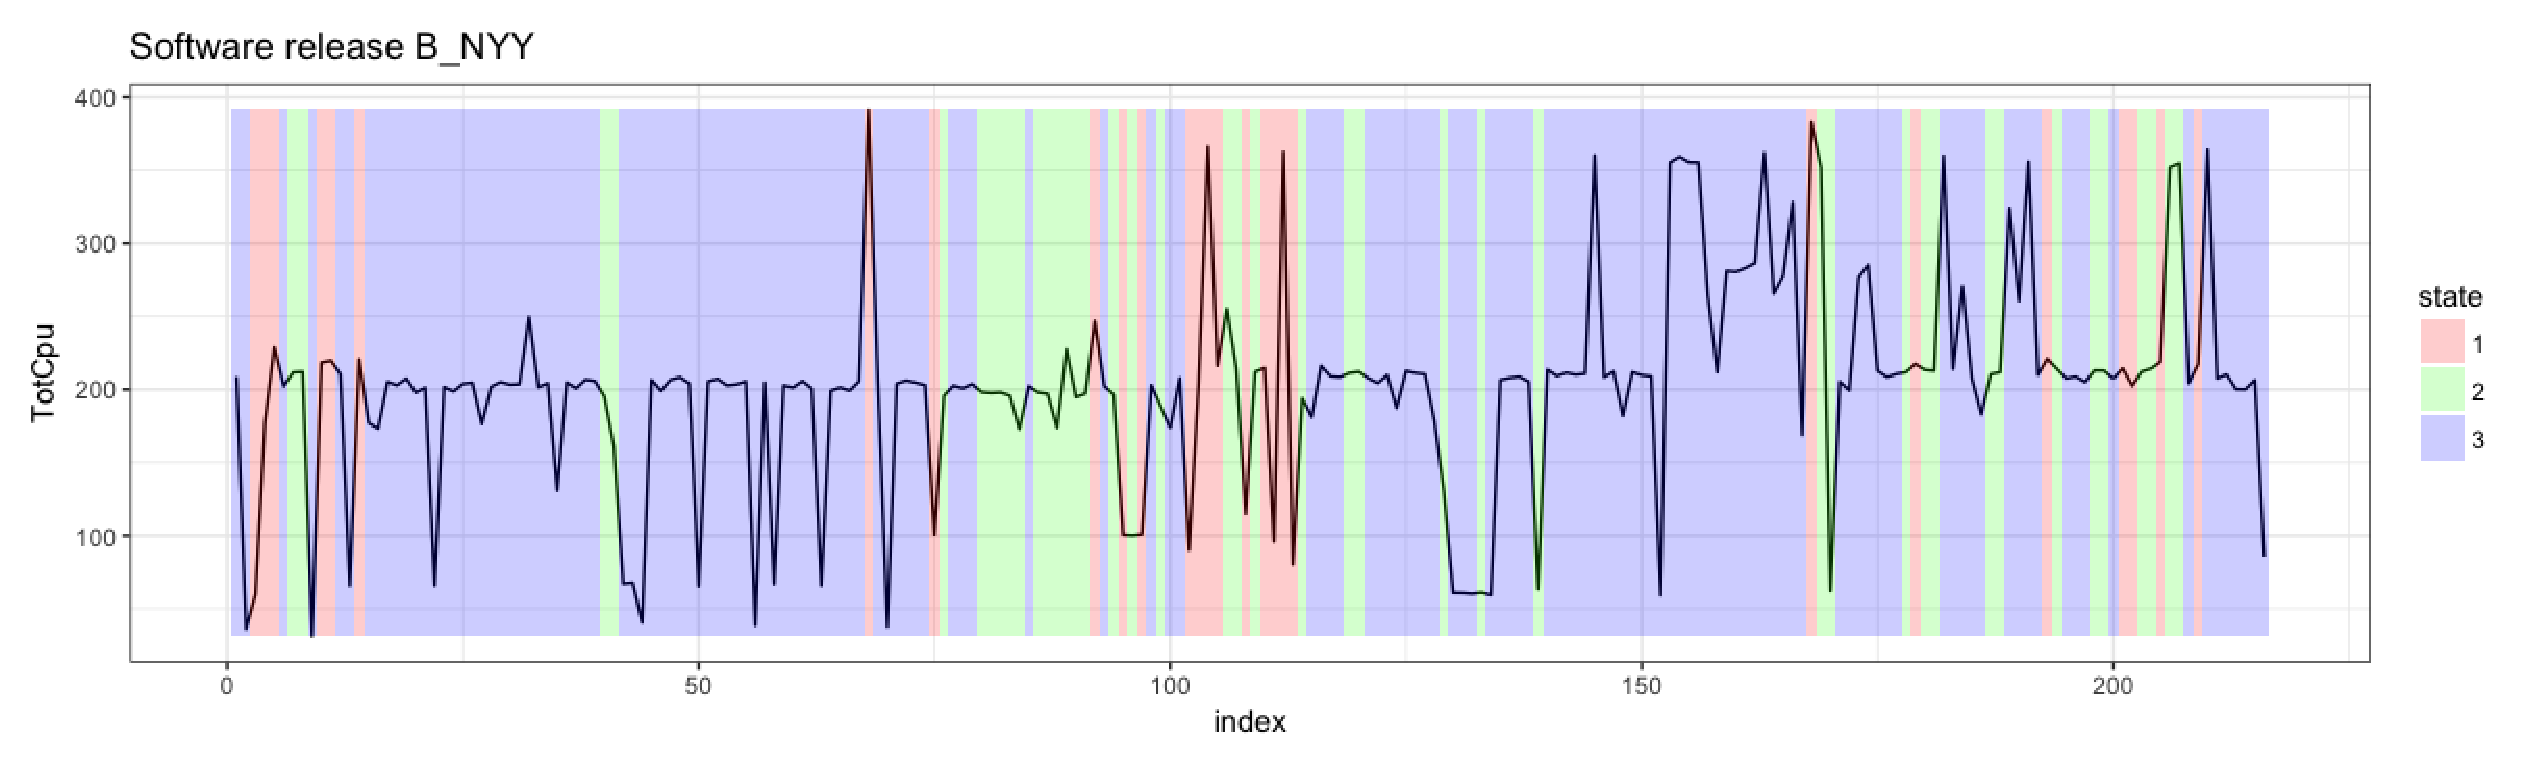
\includegraphics[width=1\linewidth]{L16B_NYY1}
	\caption{The CPU utilization showing the periods where the observation is in the specific state.}
\end{figure}

\end{frame}

%------------------------------------------------
\begin{frame}
\small{Decide: Number of switching coefficients in the model
	
Hypothesis: test environments is possible to have non-switching effects}
\rule{\textwidth}{0.4pt}

Software release L17A

\begin{figure}
	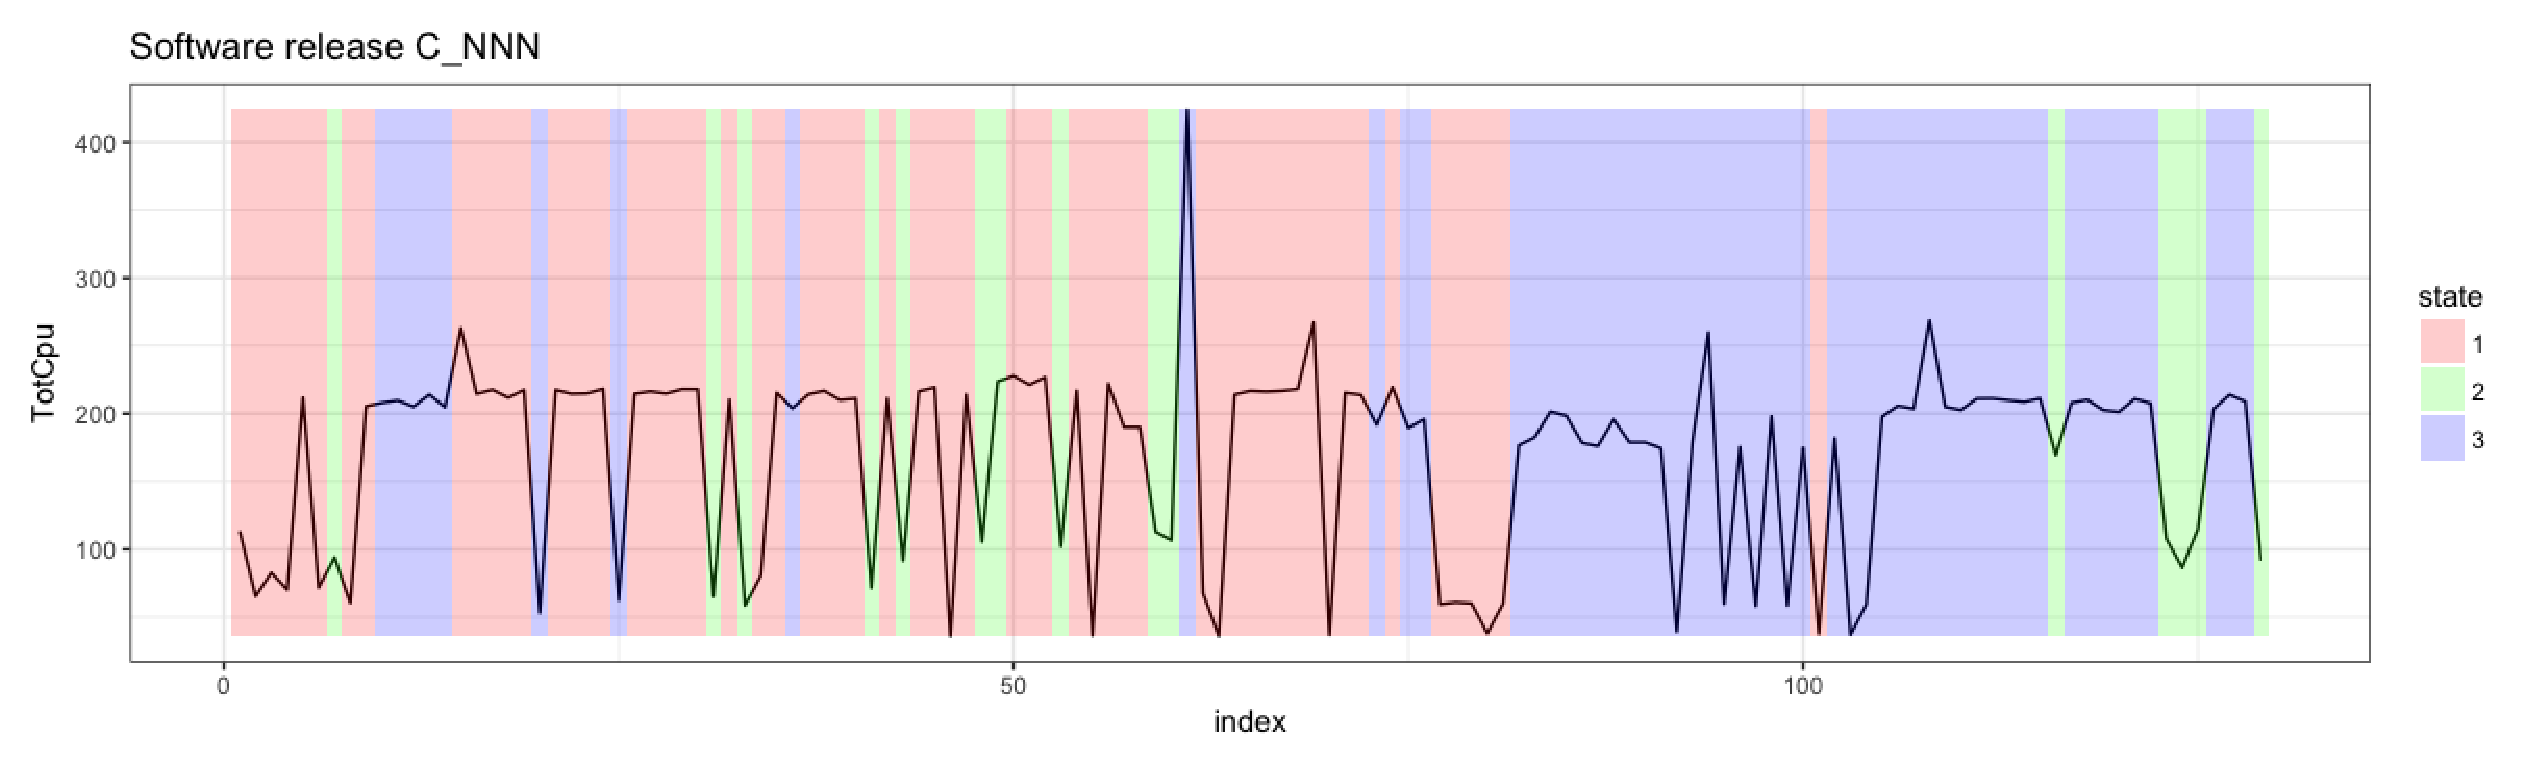
\includegraphics[width=1\linewidth]{L17A_NNN1}
	\caption{The CPU utilization showing the periods where the observation is in the specific state.}
\end{figure}

\end{frame}

%------------------------------------------------
\subsection{Comparison between the Markov switching model and the E-divisive method}
\begin{frame}
Simulated Dataset 1

\begin{figure}
	\includegraphics[width=1\linewidth]{compare_sim1}
	\caption{The simulated Dataset 1 showing the estimated change point locations}
\end{figure}

\end{frame}

%------------------------------------------------
\begin{frame}
Simulated Dataset 2

\begin{figure}
	\includegraphics[width=1\linewidth]{compare_sim2}
	\caption{The simulated Dataset 2 showing the estimated change point locations}
\end{figure}

\end{frame}

%------------------------------------------------
\begin{frame}
Real data: Software release L16A

\end{frame}
%------------------------------------------------
\begin{frame}
Real data: Software release L16B

\end{frame}
%------------------------------------------------
\begin{frame}
Real data: Software release L17A

\end{frame}

%------------------------------------------------
\section{Conclusion}
\begin{frame}
%\frametitle{Conslusion}
Concludeeeee
\end{frame}

%------------------------------------------------
\subsection{Future work}
\begin{frame}
%\frametitle{Future work}
\begin{itemize}
	\item Larger dataset
	\item Effects of other variables
	\item Consider on the other performance metrics (e.g.,memory usage and latency) 
	\item Use semi-supervised learning algorithm if some test cases are labeled with state
\end{itemize}
\end{frame}

%------------------------------------------------
\begin{frame}
\frametitle{References}
\footnotesize{
	\begin{thebibliography}{99} % Beamer does not support BibTeX so references must be inserted manually as below
		\bibitem[Hamilton, 1989]{p1} James D Hamilton (1989)
		\newblock A new approach to the economic analysis of nonstationary time series and the business cycle
		\newblock \emph{Econometrica: Journal of the Econometric Society}, pages 357-384.
	\end{thebibliography}
	
	\begin{thebibliography}{99} % Beamer does not support BibTeX so references must be inserted manually as below
		\bibitem[Sanchez-Espigares, 2014]{p2} Josep A. Sanchez-Espigares and Alberto Lopez-Moreno (2014)
		\newblock MSwM: Fitting Markov Switching Models
		\newblock \emph{CRAN R}.
	\end{thebibliography}

	\begin{thebibliography}{99} % Beamer does not support BibTeX so references must be inserted manually as below
		\bibitem[James, 2016]{p3} Nicholas A. James and David S. Matteson (2016)
		\newblock ecp: Nonparametric Multiple Change Point Analysis of Multivariate Data
		\newblock \emph{CRAN R}.
	\end{thebibliography}
}
\end{frame}

\end{document} 